%Quick Latex Template.
%Homeworks and reports. UTP-2016
%feedback:hfjimenez@utp.edu.co
\documentclass{article}									%Document class.
\usepackage[utf8]{inputenc}								%Tildes.
\usepackage{gensymb}		
\usepackage{graphicx}									%Images in the paper.
\usepackage{authblk}						
\usepackage{float}										% Image will be in the same place as you want.!!! x-/
\usepackage[table,xcdraw]{xcolor}

\title{Laboratorio 9. Experimento de Franck-Hertz}
\author{Carlos Alberto Dagua Conda, Héctor Fabio Jiménez Saldarriaga, \\Juan Camilo Castrillon\thanks{carlosdaguaco@utp.edu.co, hfjimenez@utp.edu.co, jucacastrillon@utp.edu.co} }
\date{Mayo 2016}
\begin{document}
\maketitle
\section{Abstract}
In this experimental laboratory we put in practice de Franck-Hertz  experiment which demonstrated the existence of excited states in mercury atoms, helping to confirm the quantum theory which predicted that electrons occupied only discrete, quantized energy states. Electrons were accelerated by a voltage toward a positively charged grid in a glass envelope filled with mercury vapor. Past the grid was a collection plate held at a small negative voltage with respect to the grid. The values of accelerating voltage where the current dropped gave a measure of the energy necessary to force an electron to an excited state.

\section{Introducción}
El descubrimiento de que la luz se propaga a través del espacio vacío y pueda ser emitida o absorbida por la materia solo como paquetes discretos de energía, llamados también “Cuantos de luz”, influyó profundamente sobre el estudio de la estructura de los átomos. El contenido energético de estos paquetes de energía es E = h$\upsilon$ donde \textbf{$\upsilon$} es la frecuencia de la radiación emitida y \textbf{h} la constante de Planck. \newline
Niels Bohr en 1913 contribuyo a entender la estructura atómica de la materia al proponer un modelo para el átomo cuyas predicciones fueron corroboradas posteriormente en 1914 por James Franck y Gustav Hertz quienes realizaron un experimento de bombardeo electrónico cuyos resultados estaban de acuerdo con dicho modelo y la teoría cuántica. Frank y Hertz demostraron a través del estudio de colisiones entre electrones y moléculas de gas, que la energía de interacciones atómicas está cuantizada. Por este trabajo en 1925 recibieron el premio Nobel de Física. $$\\$$ Un diagrama simplificado del experimento de Franck-Hertz se muestra en la Figura \ref{fig:diagrama}:

\begin{figure}[H]
  \centering
     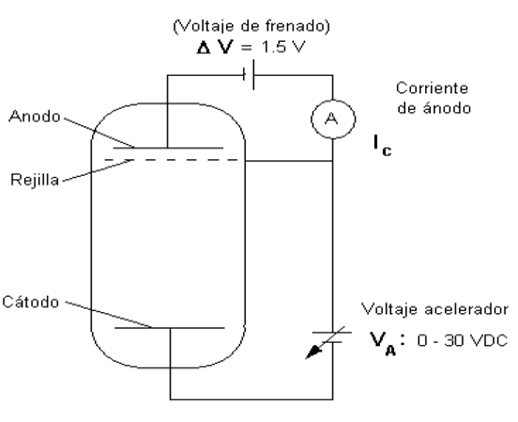
\includegraphics[width=0.7\textwidth]{diagrama}
  \caption{Representación diagrama experimental experimento \textbf{Franck-Hertz}.}
      \label{fig:diagrama}
\end{figure}
En un tubo al vacío el cual es calentado por un horno, se tiene vapor de mercurio; los electrones son emitidos por un cátodo previamente calentado y son acelerados hacia una rejilla la cual está a un potencial $V_{a}$ relativo al cátodo. Cerca de ella está el ánodo el cual está a un potencial $V_{p}$ ligeramente menor que el de la rejilla:
\begin{equation}
	V_{p} = V_{a}-D_{v}
\end{equation}
 con $D_{v} = 1.5V $

Si los electrones acelerados tienen suficiente energía cuando lleguen a la rejilla, algunos lograrán acercarse al ánodo y serán medidos como corriente $I_{c}$ por el amperímetro. Si los electrones no tienen la suficiente energía al acercarse a la rejilla serán detenidos por el potencial $D_{v}$ y quedaran en la rejilla. Así $I_{c}$ pasa a través de una serie de máximos y mínimos cuando el potencial acelerador varíe ya que $I_{c}$  crece con dicho potencial. Por tanto las moléculas del gas absorben energía de los electrones sólo cuando estos portan cantidades específicas de energía; llamadas de resonancia. Para el mercurio, el primer estado excitado es el de 4,9 $e_{V}$ por encima de su estado fundamental o base. Cuando el potencial acelerador Va de los electrones sea menor de 4,9 V, las colisiones electrón-molécula serán elásticas y los electrones no cederán energía al gas de mercurio, llegando a la rejilla con energía cinética igual a \textbf{eVa} .
\begin{figure}[H]
  \centering
     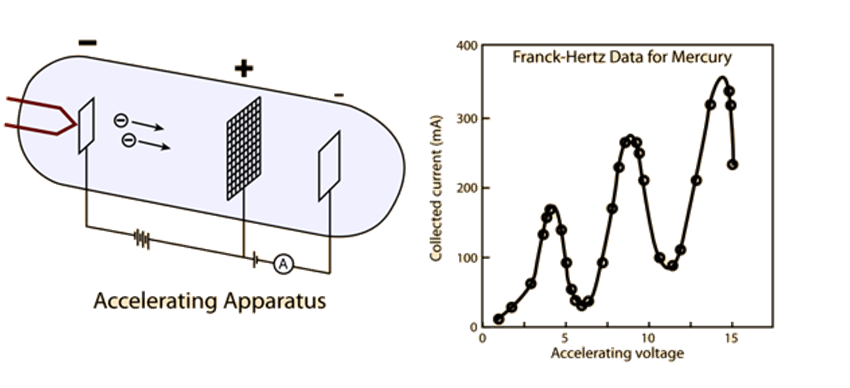
\includegraphics[width=0.97\textwidth]{grafica}
     \caption{Experimento real *Premio Nobel de Física, 1925.}
      \label{fig:grafica}
\end{figure}

Cuando $V_{a}$ sea igual a \textbf{4,9V} los electrones tendrán suficiente energía cinética para cederla en un choque inelástico con las moléculas del gas de mercurio, entonces los átomos de mercurio lo absorberán completamente los 4,9 $e_{V}$ que tienen los electrones, los cuales no tendrán energía suficiente para superar el potencial retardador $D_{v}$ y serán detenidos por la rejilla. La corriente hacia el ánodo $I_{c}$ presentara así un mínimo.\newline
$\\$
$\\$
\label{porque}
Al aumentar el potencial acelerador $V_{a}$ por encima de \textbf{4,9V},  $I_{c}$ aumentaría de nuevo; sin embargo cuando $V_{a}$ alcance 9,8 V, los electrones pueden perder toda su energía en dos colisiones con las moléculas del gas e  $I_{c}$ ser nuevamente mínima. Debido a estas múltiples colisiones inelásticas  $I_{c}$ presentara mínimos cada vez que $V_{a}$ sea múltiplo entero de \textbf{4,9V}.
$\\$
$\\$
$\\$
$\\$
$\\$
$\\$
$\\$
$\\$
$\\$
$\\$
$\\$
$\\$
\section{9.7 Análisis}
\textbf{1. Que características presenta la curva observada en el osciloscopio?}
\newline
\emph{Solución}
\newline
\begin{figure}[H]
  \centering
     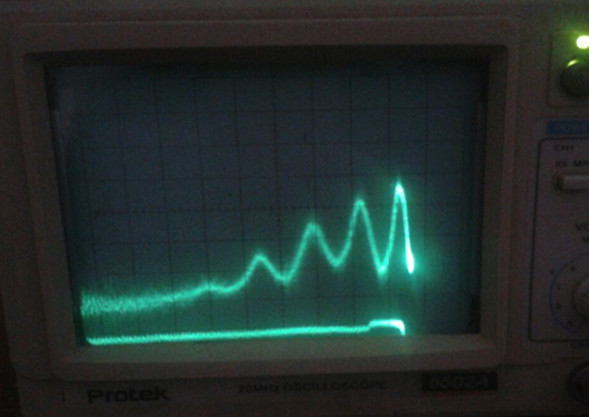
\includegraphics[width=0.8\textwidth]{osciloscopio}
  \caption{Imagen Obtenida en la practica experimental de Laboratorio.}
      \label{fig:osciloscopio}
\end{figure}
La curva representada en el osciloscopio (\textit{ver figura \ref{fig:osciloscopio}}) presenta similitud con la obtenida en el experimento de Franck y Hertz(\textit{ver figura \ref{fig:grafica2}}) , se observa que el flujo de electrones que conforman la curva presenta máximos y mínimos aproximadamente cada \textbf{4,5 eV} siendo el ideal \textbf{4,9 eV}, en cada periodo la corriente $I_{c}$ va en aumento, sin embargo, cabe recalcar que debido a dificultades técnicas, en cierta sección de la curva la corriente $I_{c}$ desciende de manera significativa.  
\newline
Se produce un cambio en el valor de un mínimo cuando varía el potencial acelerador debido a que la primera fase de 4,9 eV presenta solo un choque inelástico de las moléculas de mercurio, luego el potencial aumenta en múltiplos de 4,9 eV, es decir, aumenta hasta 9,8 eV  donde los electrones pueden perder toda su energía en dos colisiones con las moléculas del gas e $I_{c}$ puede ser nuevamente un mínimo.
$\\$
$\\$
El cambio en el valor de los máximos y de los mínimos cuando aumenta el potencial acelerador se da porque: Un mínimo se presenta cuando los electrones son capaces de excitar al mercurio y un máximo cuando cede energía cinética a los átomos de mercurio.
\begin{figure}[H]
  \centering
     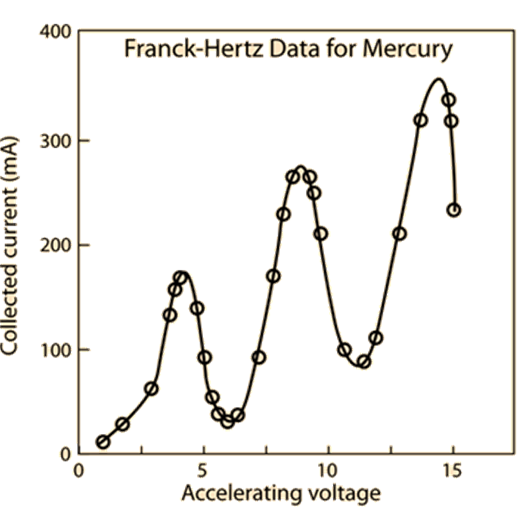
\includegraphics[width=0.75\textwidth]{grafica2}
  \caption{Representación de datos originales de Franck-Hertz muestra electrones pierden \textbf{4,9eV} por colisión con átomos de mercurio. Es posible observar diez golpes secuenciales a intervalos de 4,9 voltios.}
      \label{fig:grafica2}
\end{figure}
El significado de la diferencia de potencial entre los mínimos medidos se da cada 4.9 V en donde los electrones tienen la capacidad de producir un choque inelástico con los átomos de mercurio, esto solo se presenta cuando el potencial es un múltiplo de 4,9 V.

\textbf{2. Se produce un cambio en el valor de un mínimo cuando varía el potencial acelerador?}
\newline
\emph{Solución}
\newline
Se procedió a determinar el valor medio de los mínimos obtenidos. presentados a continuación
\begin{table}[H]
\centering
\begin{tabular}{|c|c|}
\hline
\multicolumn{1}{|l|}{Mínimos}                               & \multicolumn{1}{l|}{Voltaje {[}V{]}} \\ \hline
1                                                           & 5                                    \\ \hline
2                                                           & 4.5                                  \\ \hline
3                                                           & 4.5                                  \\ \hline
4                                                           & 4                                    \\ \hline
\begin{tabular}[c]{@{}c@{}}Voltaje \\ Promedio\end{tabular} & 4.5                                  \\ \hline
\end{tabular}
\caption{Valores de Tensión y Mínimos obtenidos}
\label{minimos}
\end{table}
El valor de un mínimo cambia cuando se varia el potencial acelerador, pues cuando este ultimo comienza desde cero y se va aumentando, la corriente aumenta hasta llegar a un máximo, en donde cede la energía cinética al átomo de mercurio; este máximo se da cuando el potencial acelerador es igual a 4.9 voltios. Estos átomos no tendrán energía suficiente para superar el potencial retardador $D_{v}$, estos átomos serán detenidos por la rejilla presentándose así un mínimo; situación que también sucede cada que $I_{c}$ sea múltiplo entero de 4.9 voltios.

\textbf{3. Por que cambia el valor de los máximos y de los mínimos cuando aumenta el potencial acelerador?}
\newline
\emph{Solución}
\newline
Cuando aumenta el potencial acelerador el valor de los mínimos y los máximos cambia porque en la primera fase que es hasta \textbf{4.9V} se presenta solo un choque inelástico de las moléculas de mercurio, donde los electrones pierden su energía presentando el primer mínimo, luego el potencial acelerador se aumenta a \textbf{9.8V} donde las moléculas de mercurio chocarán con los electrones que poseen 4.9eV, donde los otros electrones pararán con la rejilla, en la cual se presentará un segundo choque con las moléculas de mercurio, allí absorberán los 4.9 eV que poseían los electrones encontrándose así otro mínimo de $I_{c}$.

\textbf{4. Cual es el significado de la diferencia de potencial entre los mínimos medidos?}
\newline
\emph{Solución}
\newline 
La diferencia de potencial entre los mínimos representa el valor de la energía que los electrones ceden a los átomos de mercurio

\textbf{5. Determine el valor medio de la diferencia de potencial entre los mínimos medidos en la curva.}
\newline
\emph{Solución}
\newline
El valor medio de la diferencia de potencial de los mínimos medidos es de 4.5V (ver tabla \ref{minimos}).\newline 

\textbf{6. Compare este valor con el valor esperado.}
\newline
\emph{Solución}
\newline 
Sabiendo que por definición tenemos :
\begin{equation}
    \% Error = \frac{|Valor \ Teorico-Valor \ experimental|}{Valor Teorico}*100\%
\end{equation}
Si reemplazamos  en la ecuación anterior nuestros valores :
\begin{equation}
    \% Error \% = \frac{|4.9V-4.5V|}{4.9V}*100\% = \ 8.16\%
\end{equation}
Al comparar el resultado obtenido con el resultado esperado, se obtuvo un error del \textbf{8.2}\%.\newline
$$\\$$
$$\\$$

\textbf{7. Con sus datos calcule la energía de excitación del átomo de mercurio, la frecuencia y la longitud de onda correspondiente.}
\newline
\emph{Solución}
\newline 
De acuerdo a los datos obtenidos en el experimento se puede calcular la energía de excitación del átomo del mercurio, la frecuencia y la longitud de onda correspondiente para esto se tiene que:
por definición: 
\begin{equation}
E=V*h\quad ,\quad V=\frac { E }{ h } \quad 
\end{equation}
\begin{equation}
v=\frac { c }{ \lambda  } 
\end{equation}
De las ecuaciones anteriores se iguala y se despeja posteriormente $\lambda$ obteniendo:
\begin{equation}
\lambda =\frac {c* h}{ E } \qquad reemplazando \quad \textbf{E}=e*v, \quad \lambda =\frac {c* h}{ e*v}
\end{equation}
los valores que vamos a utilizar en la ecuacion anterior :
$C=3x10^{ 8 }m/s\\ h=6.625*{ 10 }^{ -34 }\quad J.s\\ e=1.6022{ 10 }^{ -19}\quad C\\ v=5,075V \\ \lambda = longitud\quad de\quad onda$
$$\\$$
\begin{equation}
\lambda=\frac { (3*{ 10 }^{ 8 })*(6.625*{ 10 }^{ -34 }) }{ (1.6022*{ 10 }^{ -19 })*4.5 } \\ \qquad \lambda=2.76*{ 10 }^{ -7 }m
\end{equation}
Hallamos entonces la energía de excitación del átomo de mercurio y la frecuencia de acuerdo a las expresiones mencionadas anteriormente tenemos:
\begin{equation}
v=\frac { c }{ \lambda  } =\frac { 3*{ 10 }^{ 8 } }{ 2.76*{ 10 }^{ -7 } } =1.087*{ 10 }^{ 15 }Hz
\end{equation}
\begin{equation}
E = h*v  \quad
E=(6.625*{ 10 }^{ -34 }J.s)*(1.087*10^{ 15 }Hz)
\end{equation}
$$\textbf{E}=7.20*{ 10 }^{ -19 }J$$

\textit{Calculo de Incertidumbres}
\textbf{8. Compare la longitud de onda hallada con el valor conocido de 253,7 nm.}
\newline
\emph{Solución}\newline
$\lambda  \textbf{hallada} = 2.76*{ 10 }^{ -7 }m$
$$\\$$
$\lambda \textbf{conocida} = 2.537*{ 10 }^{ -7 }m$
\begin{equation}
    \% Error = \frac{|Valor \ Teorico-Valor \ experimental|}{Valor Teorico}*100\%
\end{equation}
\begin{equation}
\%Error=\frac { |2.537*{ 10 }^{ -7 }m-2.76*{ 10 }^{ -7 }m| }{ 2.537*{ 10 }^{ -7 }m } *100\%=8.8\%
\end{equation}

\section{Conclusiones}
\begin{itemize}
\item El potencial acelerador obtenido en el experimento se encuentra en un rango de error de 8,16  \% sobre el valor teórico de \textbf{4,9V}.
\item El cambio en el valor de los máximos y de los mínimos cuando aumenta el potencial acelerador se da porque: Un mínimo se presenta cuando los electrones son capaces de excitar al mercurio y un máximo cuando cede energía cinética a los átomos de mercurio, se presentan cada 4,9 V aproximadamente y son en múltiplos de este último. 
\item Se determinó la longitud de onda de la primera línea de excitación de los átomos de mercurio.
\item Se estableció que no se produce un cambio en el valor de un mínimo cuando varía el potencial acelerador

\end{itemize}
\section{Bibliografia}
$[1]$ Raymond A. Serway Physics for Scientists and Engineers with Modern Physics. 
$\\$
$[2]$ http://hyperphysics.phy-astr.gsu.edu/hbase/frhz.html, The Franck-Hertz Experiment*
$\\$
$[3]$ Guía de laboratorio de física III, Universidad Tecnológica de Pereira.\footnote{Agradecimiento especial a la monitora Daniela por sus observaciones, y su gran ayuda.}

\end{document}

